\chapter{Equilibrium Statistics Applied to Chromosome Alignment}
\graphicspath{{Chapter3/Figs/}}

In previous chapter, we introduced the details of our polymer loop model for chromosomes and the simulation techniques. In this chapter, we will investigate the equilibrium statistics of the model and use the results to understand the chromosome alignment in fission yeast. 

In order to tract the model analytically, we will neglect the complex interactions such as bending energy, excluded volume effect and hydrodynamical perturbations. In another word, our model is the simplest freely-jointed polymer loop model. The transferred coordinate is utilized so that the first bead representing SPB is pinned. And an external force field will be applied. The impact of those complex interactions will be studied numerically in the chapter 5. 

We will start by introducing the setting of the model in the first section. The equilibrium statistics of 1D and 3D are discussed separately in section two and three. In the last two section, we will go back to the circumstance of fission yeast and discuss about some applications. 


%********************************** %First Section  **************************************
\section{Pinned polymer loop in a constant force field}
\label{sec:pinned_polymer_loop}
As we know, the nuclear oscillation in fission yeast is an oscillating dynamics. So in principle, the system is out of equilibrium by definition. However, notice that the time period of the nuclear oscillation is about $10$ mins. The oscillation can be divided into two parts. The chromosomes move towards to the opposite direction in each part. If the relaxation time of the system is much less than half of the oscillation period, then it is proper to think the system as a equilibrium system. Actually, we will show in next chapter that this is indeed true. The relaxation time of the chromosome system is calculated. It turns out the relaxation time scale is $\sim10$ s. So the equilibrium assumption is justified. 

\begin{figure}[htpb]
    \centering
    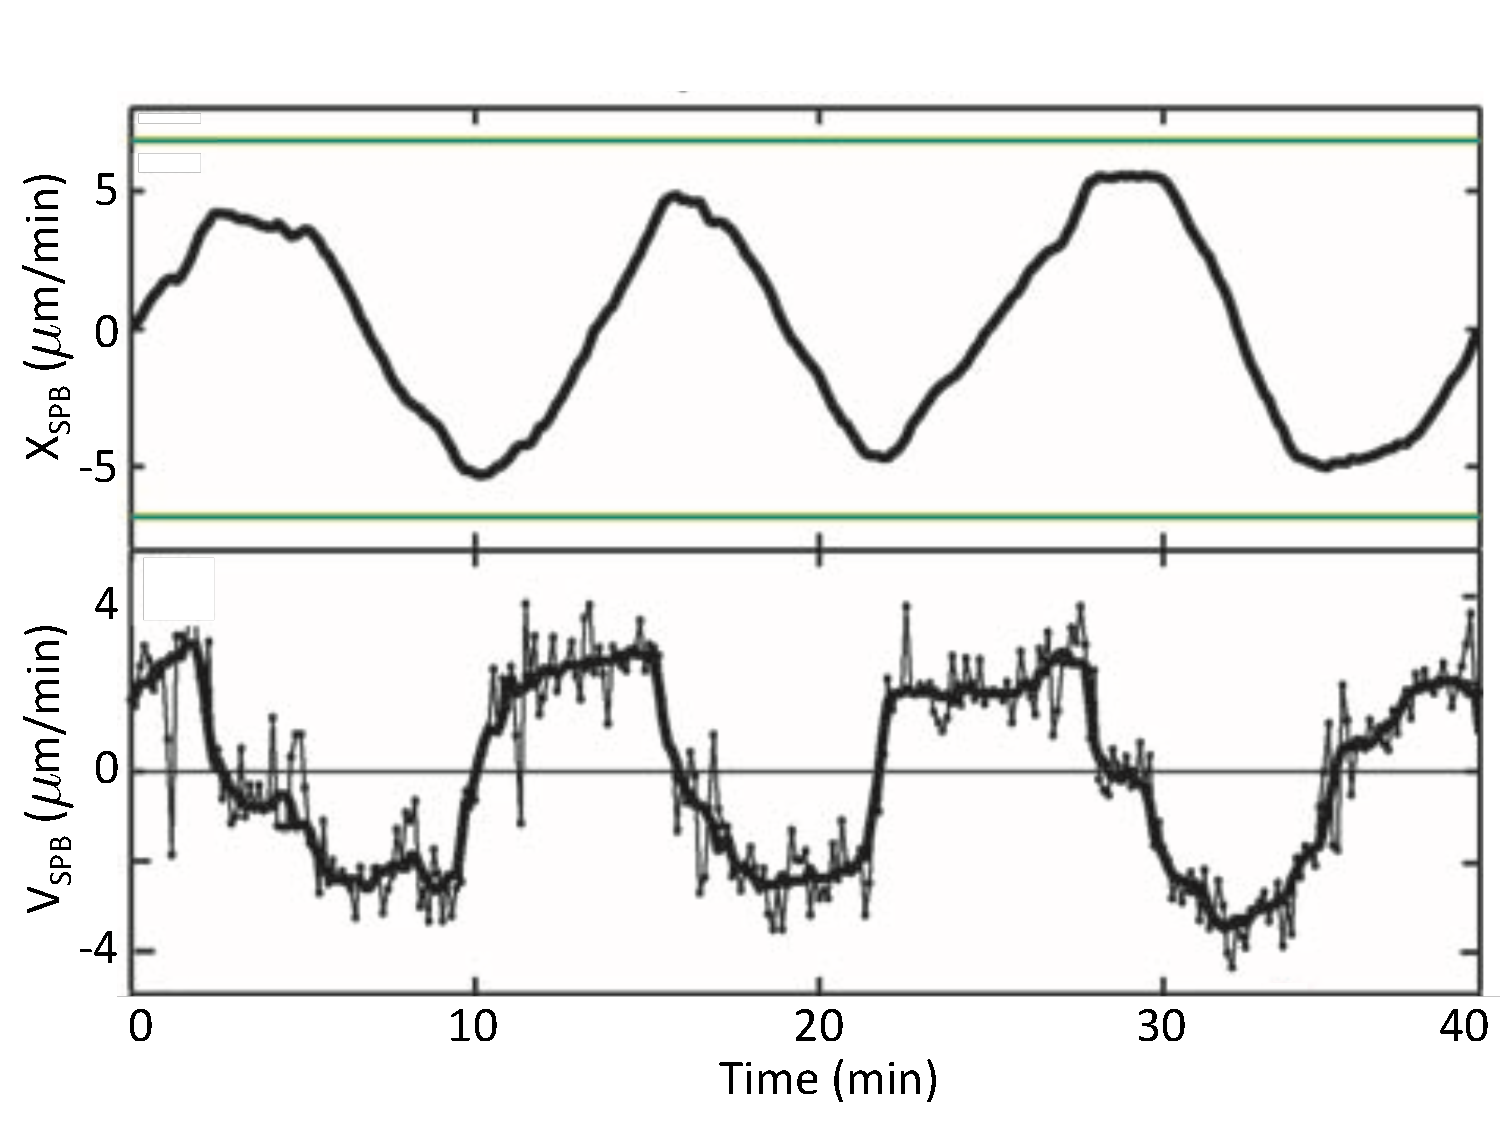
\includegraphics[width=0.8\linewidth]{vspb}
    \caption{Experimental trajectory and velocity of the SPB measured by florescence microscopy. The upper panel shows the trajectory of the SPB along the cell main axis. Green line is the boundary of the cell. The lower panel shows the corresponding velocity of the SPB. Image reprinted and modified from \cite{Vogel2009}.}
    \label{fig:vspb}
\end{figure}

On the other hand, experimental evidence shows that the velocity of the SPB is almost constant when moving towards one direction. See in Fg. \ref{fig:vspb}. So the corresponding setting of our model is pinned polymer loops in an constant external force field $\mathbf{F}=\xi v_{SPB}$. It is interesting to know what is the equilibrium statistics of this setting from theoretical point of view. In this chapter, we will use the bead-rod model to study this problem. 
\begin{figure}[htpb]
    \centering
    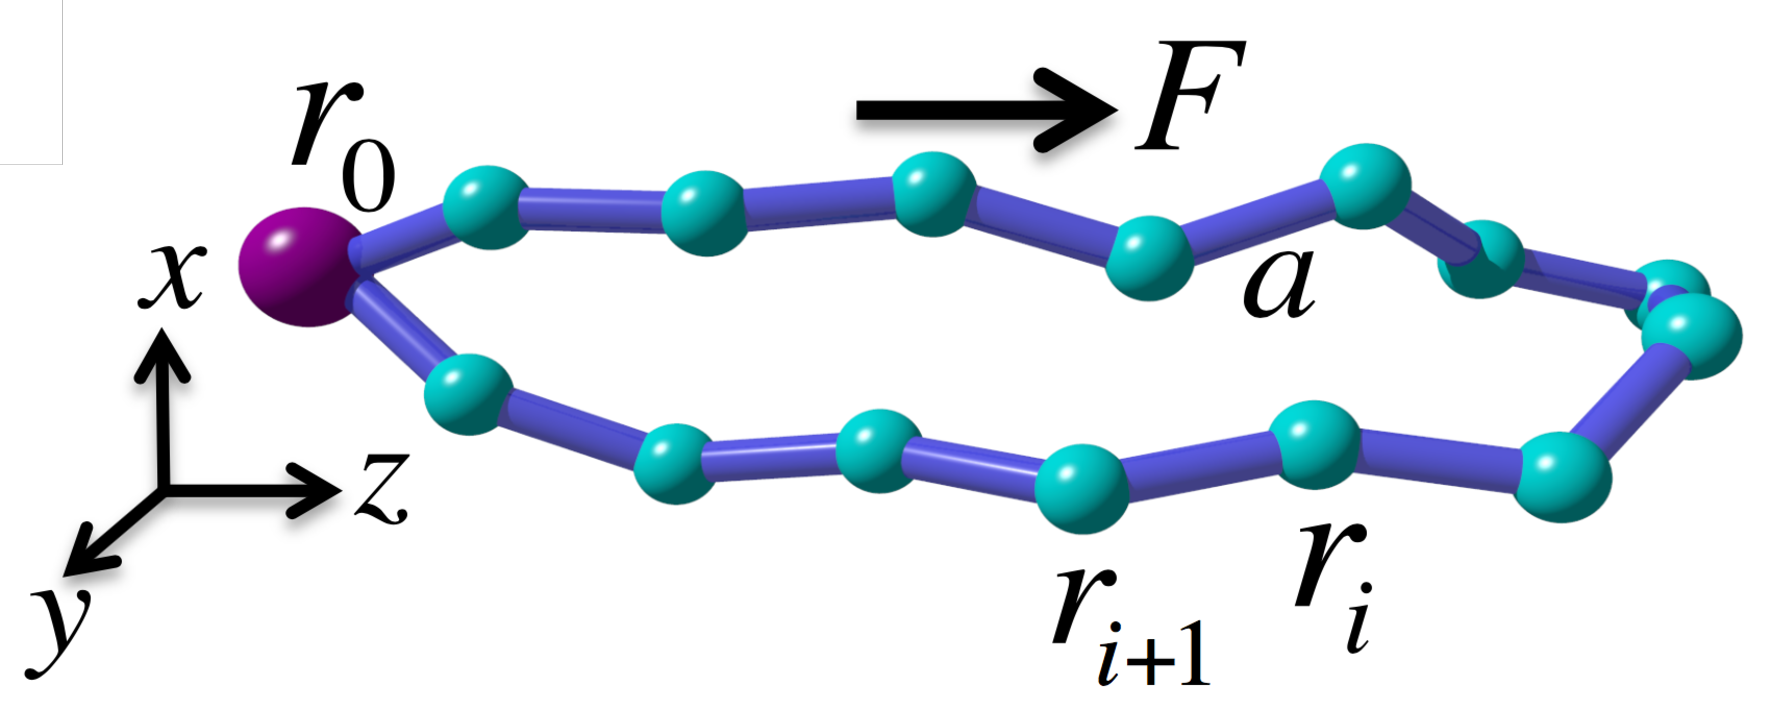
\includegraphics[width=0.7\linewidth]{beadrod}
    \caption{Sketch for the pinned bead-rod loop and notations. }
    \label{fig:beadrod}
\end{figure}

Let us first clarify some notations here. There are $L$ beads (including the SPB) in the loop and the SPB is denoted by $\mathbf{r}_0$ or $\mathbf{r}_L$ in periodic indexing. Without loss of generality, we assume it is pinned to the origin point, i.e. $\mathbf{r}_0 = \mathbf{r}_L = 0$. The length of each rod is $a$. And the constant external force field denotes by $\mathbf{F}$ is in the $z$ direction. The potential energy of the pinned polymer loop can be written as:
\begin{equation}
    \label{eq:energyBeadrod}
    E = E_0 - a\sum_{i=1}^{L} \mathbf{F}\cdot\mathbf{r}_i
\end{equation}
where $E_0$ is assumed to be a constant that denotes configuration independent energy. It is not important for the study of equilibrium statistics, we keep it here just for completeness. The orientation of the $j^{\rm{th}}$ rod is denoted by $\mathbf{u}_j = (\mathbf{r}_{j}-\mathbf{r}_{j-1})/a$. So the $i^{\rm{th}}$ bead position can be written as:
\begin{equation}
    \label{eq:beadposRodsum}
    \mathbf{r}_i = a \sum_{j=1}^{i} {u}_j.
\end{equation}
Plug it into Eq. \eqref{eq:energyBeadrod}, we arrive at
\begin{equation}
    \label{eq:energyRodsum}
    E = E_0-a\sum_{i=1}^{L}\sum_{j=1}^{i}\mathbf{F}\cdot\mathbf{u}_j.
\end{equation}
Notice that the looping condition indicates
\begin{equation}
    \label{eq:loopCondition}
    \sum_{j=1}^{L} \mathbf{u}_j = 0.
\end{equation}

In the following two sections, we will solve the equilibrium statistics in 1D first and extend the theory to 3D.


%********************************** %Second Section  *************************************
\section{Pinned Polymer Loop in 1D}
\label{sec:pinned_polymer_loop_in_1d}

As the same strategy to study many problems in physics, let us start to solve the equilibrium statistics from the simplest 1D case. The one dimensional polymer is possible because we neglect the exclusion volume effect so that the beads and rods are free to overlap. It is a simple idealized model. We will show in the following that an elegant mapping for the one dimensional pinned polymer loop to a famous classical physical model can be found. 

\subsection{Mapping to particles on 1D lattice}
\label{sub:mapping_to_particles_on_1d_lattice}

The pinned polymer in 1D is very simple. The configuration of the polymer can be specified by the orientation of the rods. In 1D, there are only two possible orientations for all rods, i.e. along the axis or against the axis. 

Let us denote the $j^{\rm{th}}$ rod orientation by $u_j\in\{-1, +1\}$, where $u_j = +1$ means the rod orientates along the axis and $u_j = -1$ means the rod orientates against the axis. Again the $i^{\rm{th}}$ bead position in 1D is $z_i = a\sum_{j=1}^{i}u_j$. Now let us introduce a shifted and rescaled variable 
\begin{equation}
    \label{eq:variableu2n}
    n_j = (u_j + 1)/2. 
\end{equation}
We can easily find that $n_j\in\{0,1\}$. The configuration of the 1D polymer can be denoted by $\{n_1, n_2, \cdots, n_L\}$. Since $n_j$ is a binary variable, we can interpret $n_j = 1$ as a lattice site occupied by a particle, and $n_j = 0$ as an empty lattice site. In this way, we find a one-to-one mapping from the configuration of polymers to particles on lattice sites. See in Fig. \ref{fig:mapping}. The number of rods equals to the number of lattice sites. Without loss of generality, we have shown in the figure the right-orientated rod corresponds to an occupied site, and the left-oriented rod corresponds to an empty site.

\begin{figure}[htpb]
    \centering
    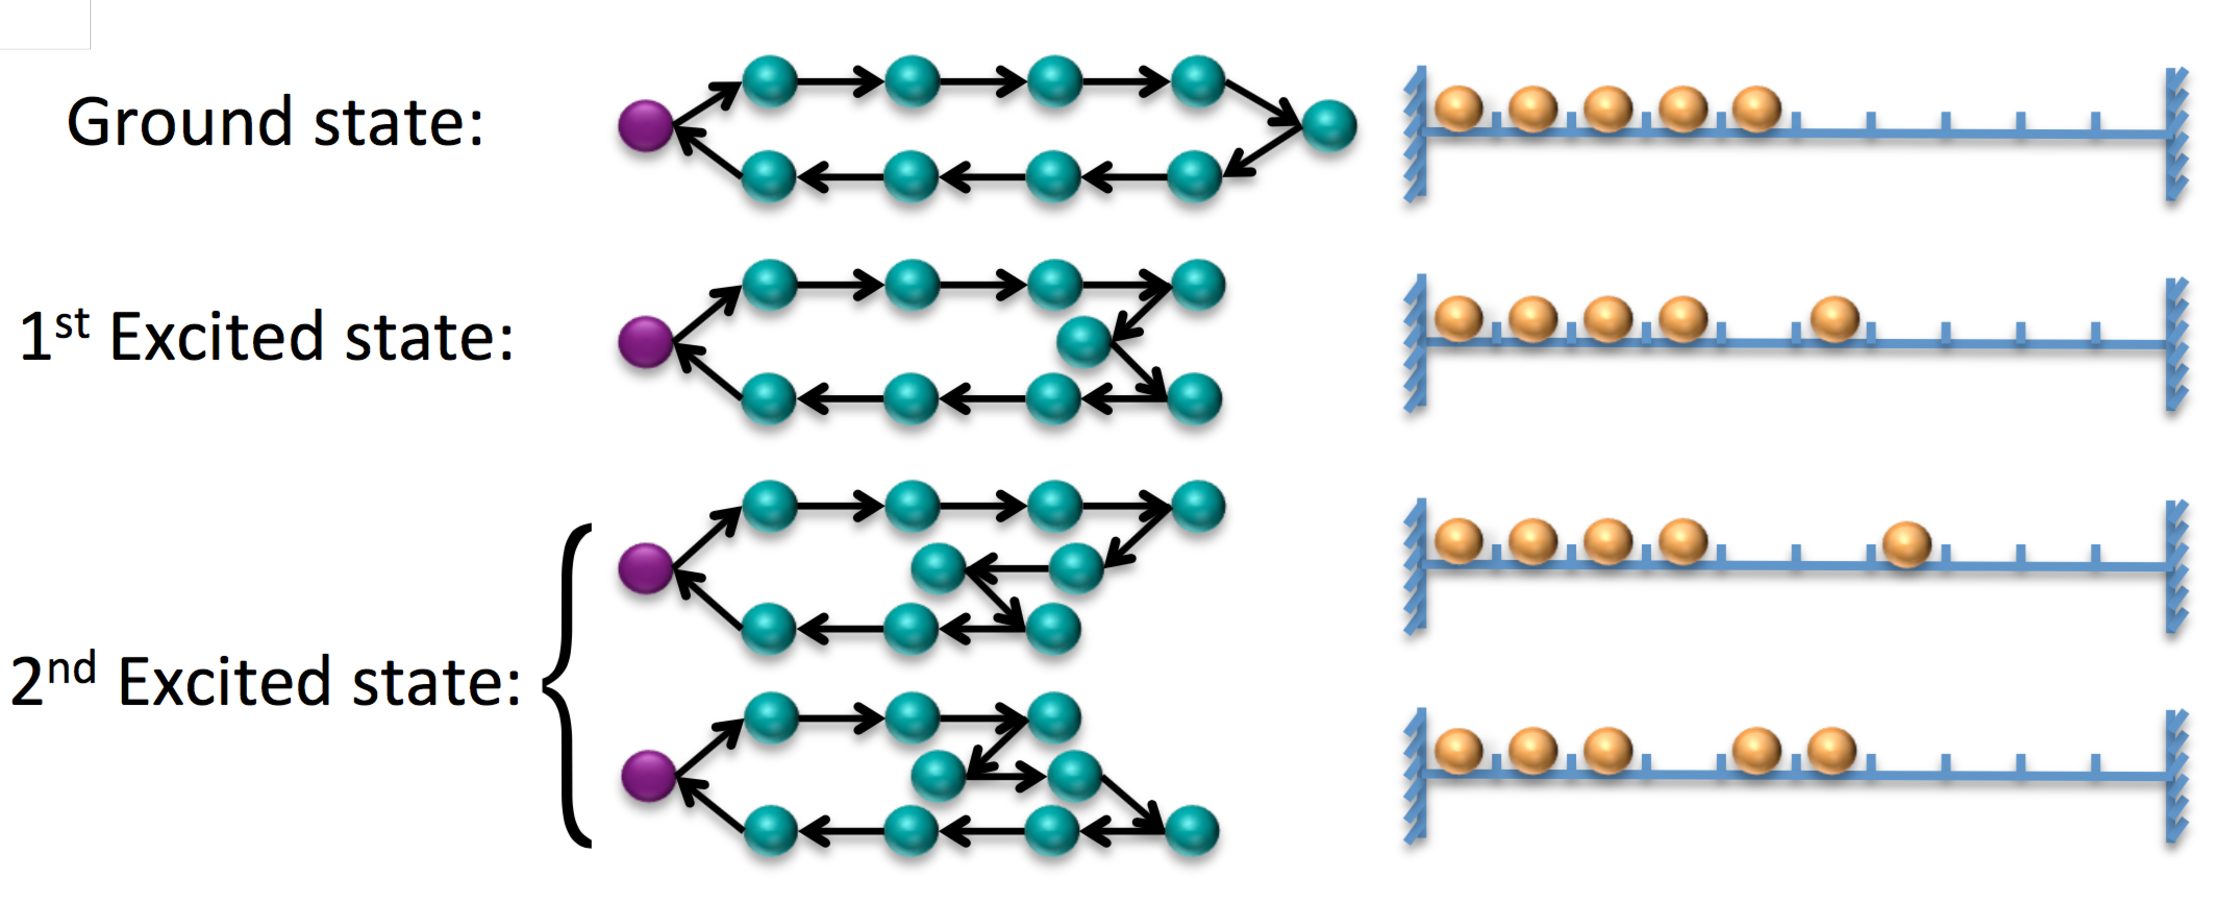
\includegraphics[width=0.9\linewidth]{mapping}
    \caption{Illustration for the mapping from 1D pinned polymer loop to Fermionic particles on 1D lattice sites. }
    \label{fig:mapping}
\end{figure}

Here are some remarks for the mapping:

$\bullet$ The mapped particles are exclusive to each other. It is not possible for one lattice occupied by more than one particles. In another word, these particles are Fermions. This is because the system is a two state system, there is no correspondent polymer state for a site occupied by more than one particle.

$\bullet$ According to the looping condition Eq. \eqref{eq:loopCondition}, the total number of rods pointing to the right must be exact $L/2$. Correspondingly, the total number of particles also must be exact $L/2$, i.e.
\begin{equation}
    \label{eq:loopConditionParticle}
    \sum_{j=1}^{L}{n_j} = \frac{L}{2}.
\end{equation}
Furthermore, the number of particles must be conserved during the change of configurations.

$\bullet$ The dynamics of 1D polymer can be mapped to the particle hopping process on the 1D lattice. This part will be discussed in next chapter.

$\bullet$ The mapping is essentially from a two state system to a two state system. One can also interpret the two state as spin up and spin down or any other two state systems. We use the particle-lattice interpretation because it is familiar and intuitive to most people. 

Now let discuss the energy of the system. Rewrite Eq. \eqref{eq:energyRodsum} in 1D we get
\begin{equation}
    \label{eq:energyRodsum1D}
    E = E_0 - Fa \sum_{i=1}^L\sum_{j=1}^i u_j.
\end{equation}
Exchange the summation order in Eq. \eqref{eq:energyRodsum1D} and utilizing the loop condition $\sum_{j=1}^L u_j = 0$ we obtain
\begin{equation}
    \label{eq:energy1D}
    E = E_0 + Fa \sum_{j=1}^L j u_j.
\end{equation}
Let us look at the energy from the particle-lattice picture. Substitute Eq. \eqref{eq:variableu2n} into Eq. \eqref{eq:energy1D}, we arrive at
\begin{equation}
    \label{eq:energy1DRewrite}
    E = \tilde{E}_0+\Delta E\sum_{j=1}^{L} j n_j 
\end{equation}
where $\Delta E = 2Fa$ and $\tilde{E}_0 = E_0 - L(L+1)\Delta E/4$ is the unimportant energy offset. Let us ignore the offset in our discussion. Eq. \eqref{eq:energy1DRewrite} can be reinterpret as the summation energy of $L$ lattice sites. When $n_j = 1$ (occupied site), we gain a energy of $j\Delta E$ and zero otherwise. One can clearly see that Eq. \eqref{eq:energy1DRewrite} is the energy of a system of $L/2$ fermions distributed over $L$ equidistant energy levels $\Delta E, 2\Delta E, \cdots, L\Delta E$.
The lowest energy (ground state) corresponds to the configuration that the left half of lattice sites are fully filled by particles. And the corresponding polymer picture is the fulled stretched configuration. The correspondence of the $1^{\rm{st}}$ and the $2^{\rm{nd}}$ excited states also can be imagined, which is shown in Fig. \ref{fig:mapping}. 

The mapping from the polymer to the particle-lattice picture is very useful for searching the solution of equilibrium statistics. In the following subsections, we will solve the 1D statistics using two different methods. The first one based on the grand canonical ensemble is an approximate solution with a simpler formulism, while the second one is the exact solution based on the canonical ensemble but a more complex formulism. We will calculate the mean position of beads and their variance. Because these are what we interested, the biological interactions can only happen when two segments are closer enough. 

\subsection{The grand canonical ensemble solution}
\label{sub:the_grand_canonical_ensemble_solution}
We have mentioned in the previous subsection that the particle number is conserved to $L/2$ in the mapped particle-lattice picture. So in principle, the system is a canonical ensemble system. However, let us first release this constraint by allowing the particles exchange with the reservoir at both sides of the lattice. Thus the grand canonical ensemble can be applied. After that, we can reimpose the constraint using the Brownian bridge technique. We can obtain very accurate mean bead position and its variance use this method. Given that the formulation of this method is simple, we are quite satisfied with the results. Let us now illustrate the method in details.

\subsubsection{The Fermi-Dirac statistics}
\label{ssub:The Fermi-Dirac Statistics}

As we have mentioned above, the particles on the lattice are Fermions. One wonderful thing of the grand canonical ensemble is the particles can be assumed to be mutually independent. So that we can directly use the famous \emph{Fermi-Dirac} distribution. That is to say the probability of a lattice site is occupied can be written as
\begin{equation}
    \label{eq:fermiDirac}
    \mathbb{P}\{n_j=1\} = \frac{1}{1+\exp\left[\frac{\Delta E (j - \mu)}{k_B T}\right]},
\end{equation}
where $\mu$ is the chemical potential $\mu = (L+1)/2$ obtained from the requirement that on average there are $L/2$ particles in the system. And accordingly, the probability that a lattice site is empty writes
\begin{equation}
    \label{eq:probEmpty}
    \mathbb{P}\{n_j=0\} = 1 - \mathbb{P}\{n_j=1\}.
\end{equation}
Let us define a dimensionless quantity which we call it \emph{dimensionless temperature}:
\begin{equation}
    \label{eq:dimensionlessT}
    \tilde{T} = \frac{k_B T }{\Delta E} = \frac{k_B T}{2Fa}
\end{equation}
Now we can see in Fig. \ref{fig:fermiDirac} for an illustration of the \emph{Fermi-Dirac} distribution of different $\tilde{T}$. When $\tilde{T}$ is small, namely the external force is large, the distribution shows a strong bias. The left half sites are more likely to be occupied and the right half sites are more likely to be empty. In the polymer picture, this means the orientation of the first half rods is biased in the direction of force, whereas the second half of rods are more probable to point against the force field. Physically, it is easy to understand because the pinned polymer in strong force field is almost stretched.

\begin{figure}[htpb]
    \centering
    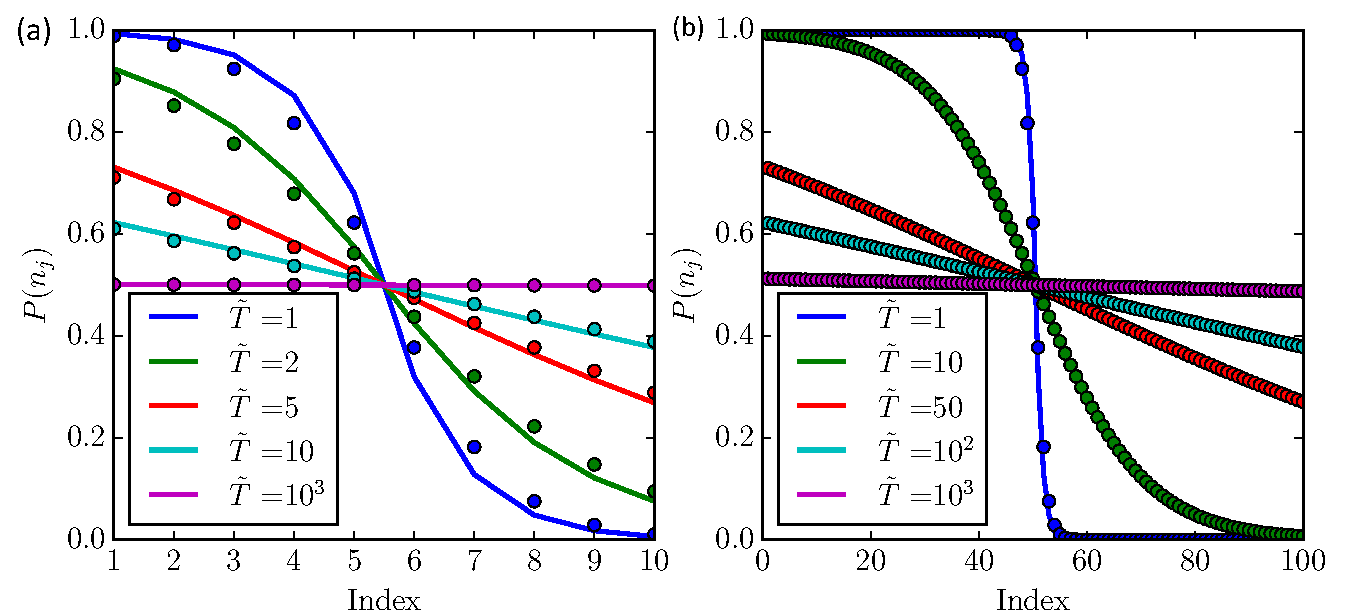
\includegraphics[width=1.0\linewidth]{fermiDirac}
    \caption{Fermi-Dirac distribution compared with the exact solution from the number partition theory. Solid lines are the exact solution while the dots are Fermi-Dirac approximations. Different dimensionless temperature is indicated by different colors as shown in the legend. (a) $L=10$, (b) $L=100$. }
    \label{fig:fermiDirac}
\end{figure}

With Eq. \eqref{eq:fermiDirac}, the mean and variance of random variable $n_j$ can be calculated straightforwardly:
\begin{subequations}
    \begin{align}
        \label{eq:nmean}
        \left<n_j\right> & = \mathbb{P}\left\{n_j=1\right\},\\
        \label{eq:nvar}
        \text{var}\left[n_j\right] & = \mathbb{P}\left\{n_j=1\right\} \cdot \mathbb{P}\left\{ n_j=0\right\} 
        - \left<n_j\right>^2.
    \end{align}
\end{subequations}
On the other hand, from Eq. \eqref{eq:beadposRodsum} and Eq. \eqref{eq:variableu2n} we can calculate the position of bead as
\begin{equation}
    \label{eq:beadpos1D}
    z_i = a\left(2\sum_{j=1}^i n_j - i\right).
\end{equation}
If we assume $n_1, n_2, \cdots, n_L$ are all mutually independent, then the mean and variance of bead position can simply calculated as
\begin{subequations}
    \label{eq:meanVarPos1D}
    \begin{align}
    \label{eq:meanPos1D}
        \left<z_j\right> & = a \left(2\sum_{j=1}^i \left<n_j\right> - i\right),\\
    \label{eq:varPos1D}
        \text{var}\left[z_j\right] & = 4a^2\sum_{j=1}^i\text{var}\left[n_j\right]
    \end{align}
\end{subequations}
The results of the above equations can be compared to the Monte-Carlo simulation (see Appendix \ref{append:mc1D} for details). 
We found that the formula for mean bead position works perfect. However, the formula for variance does not work so good. Notice that Eq. \eqref{eq:varPos1D} is monotonically increasing with the index $i$. We can take the simple symmetric argument that the $\text{var}\left[z_i\right] = \text{var}\left[z_{L-i}\right]$. The result after that still can not match with the simulations. See in Fig. \ref{fig:meanVarAdd1D}.

\begin{figure}[htpb]
    \centering
    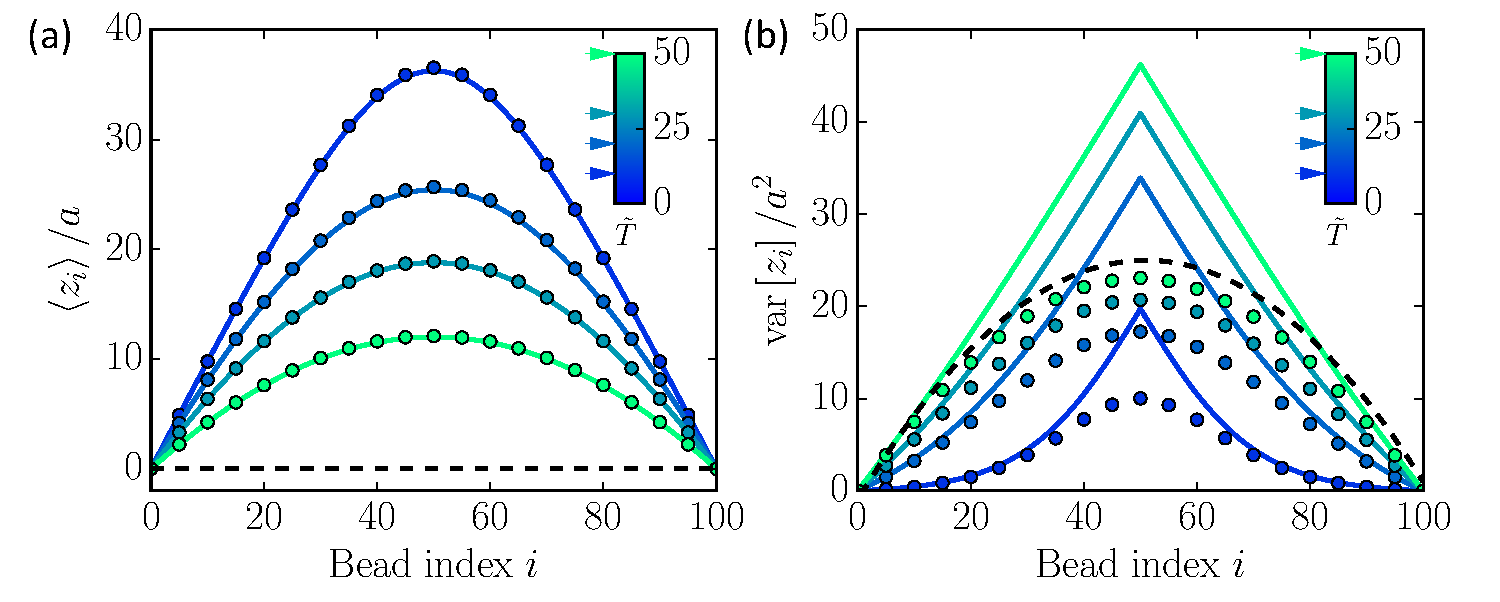
\includegraphics[width=1.0\linewidth]{meanVarAdd1D}
    \caption{Mean and variance of the 1D pinned polymer bead positions. MC simulation results (dots) are compared with theoretical results (solid lines) Eq. \ref{eq:meanVarPos1D}. The length of the polymer loop $L=10$. The black dash line indicates the case $\tilde{T}\rightarrow\infty$, i.e. no external force field. }
    \label{fig:meanVarAdd1D}
\end{figure}

The reason for this mismatch is simple, the particles are not exactly independent and the loop condition is only fulfilled on average by choosing the chemical potential $\mu=(L+1)/2$ in Eq. \eqref{eq:fermiDirac}. In the following part, we will show how to solve this problem use the Brownian bridge technique. 

\subsubsection{The Brownian bridge condition}
\label{ssub:The Brownian Bridge Condition}
Let us consider the polymer loop as a random walk that returns to the origin point after $L$ steps. This sort of random walk process is called the Brownian bridge \cite{Feller2008,Athreya2006}. So each rod represents a random walk step. The segment connecting the $k^{\rm{th}}$ and the $l^{\rm{th}}$ bead corresponds to the propagator $\rho(z_l = z | z_k=0)$. According to the Lindeberg-Feller central limit theorem \cite{Feller2008}, this propagator is Gaussian with the mean and variance equal to the sum of the mean and variance of all individual steps from $k$ to $l$.

As we said above, the grand canonical ensemble only ensures the loop condition on average. To solve the problem, we now impose the Brownian bridge condition so that every single trajectory fulfills the loop condition. The Brownian bridge can be formulated as following:
\begin{equation}
    \label{eq:brownianBridge}
    \rho^L(z_i=z) = \frac{\rho(z_i=z|z_0=0)\rho(z_{L-i}=z|z_L=0)}{\rho(z_L=0|z_0=0)},
\end{equation}
where $\rho(z_i=z)$ is the probability density function of finding the $i^{\rm{th}}$ bead at position $z$, $\rho(z_k=z|z_j=0)$ are the propagators. Eq. \eqref{eq:brownianforce} means that the probability density equals two pieces of random walk trajectory of length $i$ and $L-i$ meet at position $z$ on the condition that they are belong to the same loop. 

Notice that the propagators are Gaussian with the variance added up by the variance of individual steps, i.e Eq. \eqref{eq:varPos1D}. So that $\rho^L(z_i = z)$ is also Gaussian. Its variance is given by
\begin{equation}
    \label{eq:varBrownianBridge}
    \text{var}\left[z_i\right] = 4a^2\frac{\sum_{j=0}^{i}\text{var}\left[n_j\right]\sum_{j=L-i}^{L}\text{var}\left[n_j\right]}{\sum_{j=0}^{L}\text{var}\left[n_j\right]}.
\end{equation}
Plug in Eq. \eqref{eq:nvar} and Eq. \eqref{eq:varPos1D} we can obtain the variance of bead position in the loop. For $\tilde{T}\gg 1$, we can obtain the close form expressions for mean and variance of bead position by converting the summation to integral
\begin{subequations}
    \label{eq:meanVarPos1DExpression}
    \begin{align}
        \left< z_i \right> & = 2 a \tilde{T} \ln\left[ \frac{1+\exp\left(\frac{L}{2\tilde{T}}\right)}{\exp\left(\frac{i}{2\tilde{T}}\right) + \exp\left(\frac{L-i}{2\tilde{T}}\right)} \right] \\
        \text{var}\left[z_i\right] & = 2 a^2 \tilde{T} \frac{ \sinh\left( \frac{L-i}{2\tilde{T}}\right) \sinh\left( \frac{i}{2\tilde{T}}\right)} {\sinh\left( \frac{L}{2\tilde{T}}\right) \cosh^2\left( \frac{L-2i}{4\tilde{T}}\right)}
    \end{align}
\end{subequations}
We can see from the above formulas that the $z_i-z_{L-i}$ symmetry is satisfied. And a strong external force field leads to a stretched configuration and a small fluctuation of bead position. This result is compared with the Monte-Carlo simulations, see in Fig. \ref{fig:meanVar1D}.

\begin{figure}[htpb]
    \centering
    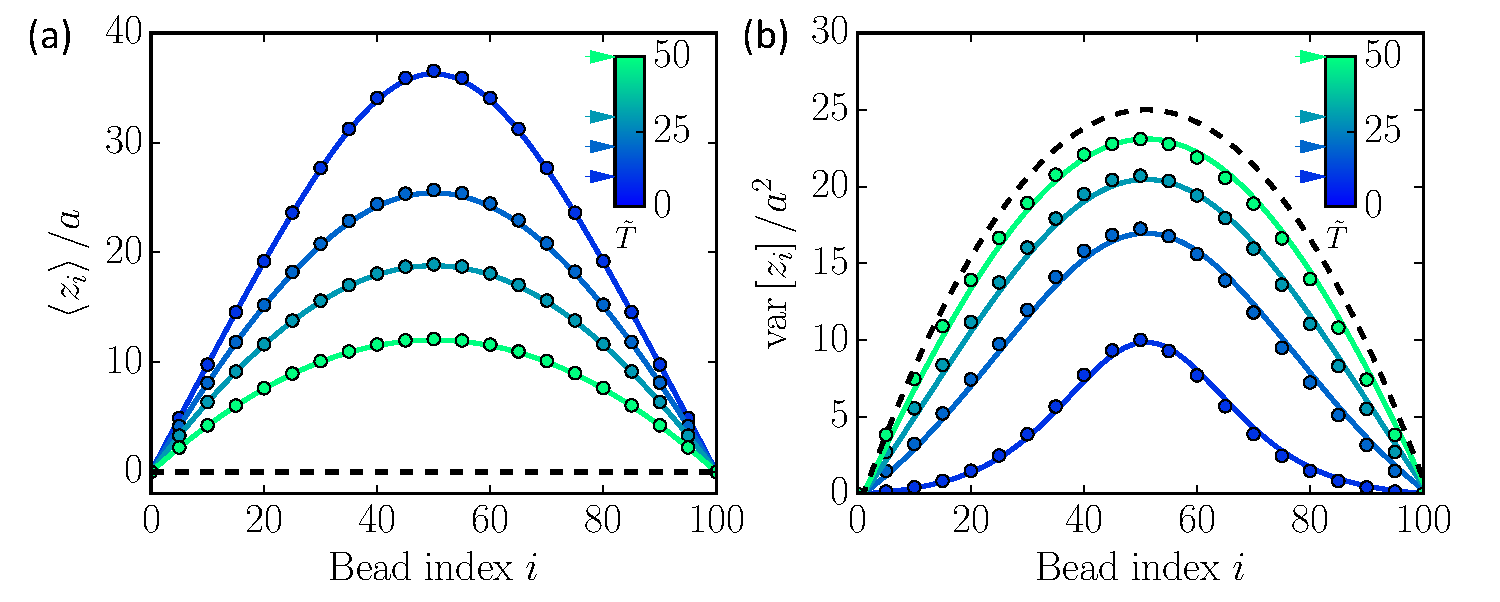
\includegraphics[width=1.0\linewidth]{meanVar1D}
    \caption{Mean and variance of the 1D pinned polymer bead positions. MC simulation results (dots) are compared with theoretical results (solid lines) Eq. \ref{eq:meanVarPos1DExpression}. The length of the polymer loop $L=10$. The black dash line indicates the case $\tilde{T}\rightarrow\infty$, i.e. no external force field. }
    \label{fig:meanVar1D}
\end{figure}

In this subsection, we solved the mean and variance of bead position for 1D pinned polymer loop in an external force field. The strategy is using the \emph{Fermi-Dirac} statistics and re-enforce the loop condition by the Brownian bridge technique. Excellent results verified by the Monte-Carlo simulation are obtained. However, we have to say, this is just an approximate method. In the next subsection, we will use the canonical ensemble to obtain the exact solution. 

\subsection{Canonical ensemble solution}
\label{sub:canonical_ensemble_solution}
In the particle-lattice picture, the system is actually a canonical ensemble system because of the conservation of particle number. In this section, we will calculate the exact partition function using this ensemble. More interestingly, we will show the calculation can be recoded to a number partition problem. Exact results are obtained and compared with the results from the approximate approach above.

\subsubsection{The number partition theory}
\label{ssub:The Number Partition Theory}
Before the calculation of exact partition function, let us discuss an interesting number partition problem that share a lot of similarities with the former. 

Consider a non-negative integer number $K$, which can be expressed into the summation of $N$ non-negative integers:
\begin{equation}
    K = \sum_{j=1}^N k_j
\end{equation}
However, there is a constraint on the summation components $0 \leqslant k_1 \leqslant k_2 \cdots \leqslant k_N \leqslant M$. This kind of problem can be best visualized by what called Young diagram \cite{Andrews1998}, shown in Fig. \ref{fig:young}.
\begin{figure}[htpb]
    \centering
    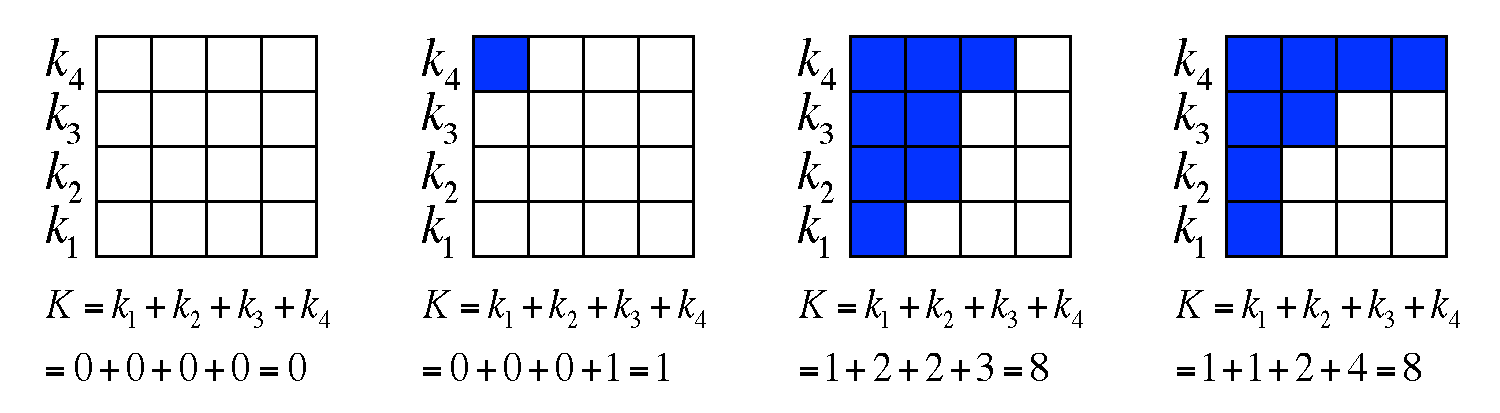
\includegraphics[width=1.0\linewidth]{young}
    \caption{Some examples of the Young diagram.}
    \label{fig:young}
\end{figure}
In the Young diagram, each row represents a integer number. The number of blue boxes means the value of the $j^{\rm{th}}$ integer. Starting from the bottom, because of the constraint, the diagram is non-decreasing. 

The question is, given a certain integer $K$, how many different ways are there to partition it into $N$ non-decreasing pieces $\{k_1, k_2, \cdots, k_N\}$. For the simple cases, one can tell the answer immediately. For examples, in the first two examples of Fig. \ref{fig:young}, we illustrate that there are only one way to partition integer $0$ or $1$ into $4$ non-decreasing integers. However, this question in the general case is not intuitive. Fortunately, this problem is well studied by mathematicians. Let $g(M, N; K)$ denote the number of partitions of $K$ with at most $N$ parts, each of size at most $M$. Equivalently, these are the partitions whose Young diagram fits inside an $N \times M$ rectangle. Then we have the following generating function:
\begin{equation}
    \label{eq:generatingDegeneracy}
    \Phi(q):=\sum_{K=0}^{MN} g(M, N; K) q^K = \binom{M+N}{N}_q
\end{equation}
where $q$ is an auxiliary number, and the notation at the right hand side of Eq. \eqref{eq:generatingDegeneracy} is called $q$ binomial coefficient or Gaussian binomial coefficient. It is defined as 
\begin{equation}
    \label{eq:qBinomial}
    \binom{L}{N}_q := \frac{[L]_q!}{[L-N]_q![N]_q!},
\end{equation}
and $[N]_q := 1 + q + q^2 + \cdots + q^{N-1}$ is called a $q$ number \cite{Andrews1998}.


\subsubsection{Exact partition function}
\label{ssub:Exact Partition Function}
Now, let us start to calculate the partition function of our pinned polymer in the particle-lattice picture. The partition function of a canonical ensemble system with discrete energy can be written as:
\begin{equation}
    \label{eq:partitionFuncCanonical}
    \mathcal{Z}\left(T\right) = \sum_{E}g(E)\exp \left(-\frac{E}{k_B T}\right),
\end{equation}
where $g(E)$ is the degeneracy of the microscopic states which have the same energy $E$. Once $g(E)$ is known, the partition function can be calculated straightforwardly.

Let us take a look at the energy of the system, i.e. Eq. \eqref{eq:energy1DRewrite}. It is represented in the way of rod orientation $u_j$ or occupation variable $n_j$. Here, we are going to use another way to represent the energy. In the particle-lattice picture, the system consists $N:=L/2$ particles. So the energy can be rewritten as:
\begin{equation}
    E = \tilde{E}_0 + \sum_{j=1}^N E_j,
\end{equation}
where $E_j$ is the energy of the $j^{\rm{th}}$ particle in the external force field. Again, $\tilde{E}_0$ is an unimportant constant energy offset. Denote the position of the $j^{\rm{th}}$ particle as $x_j$, which is an integer $x_j\in[1, L]$. Then we can write $E_j = x_j \Delta E$. 
Also notice that, because of the exclusive condition, the sample space of the particle system is constrained in $\Omega = \{\mathbf{x}| 1\leqslant x_1<x_2<\cdots<x_N\leqslant L\}$.

Let us do a shift for the particle position by defining
\begin{equation}
    k_j := x_j - j.
\end{equation}
Notice now the constraint on $x_j$ is transferred to $0 \leqslant k_1 \leqslant k_2 \cdots \leqslant k_N \leqslant N$. And the energy of the system can be rewritten as:
\begin{equation}
    E = \hat{E}_0 + \Delta E \sum_{j=1}^N k_j = \hat{E}_0 + K \Delta E,
\end{equation}
Again $\hat{E}_0$ here is an unimportant constant energy offset, $\hat{E}_0 = \tilde{E}_0+N(N+1)/2$. 
It is not difficult to find the range of the energy is $\hat{E}_0, \hat{E}_0 + \Delta E, \cdots, \hat{E}+N^2\Delta E$. 

Now we are closer to the number partition problem. Notice that $K=\sum_{j=1}^{N}k_j$ and we have the same type of constraint as in the number partition problem. In addition, because the mapping from integer $K$ to energy $E$ is one-to-one. So the degeneracy function $g(E)$ is exactly the number of ways to partition the integer $K$. Furthermore, let us denote $q:=\exp\left(-\Delta E/ k_B T\right)$. Then we have
\begin{equation}
    \begin{aligned}
    \label{eq:partitionFuncExact}
    \mathcal{Z}\left(T\right) & = \sum_{E}g(E)\exp \left(-\frac{E}{k_B T}\right) \\ 
    & = \exp\left(-\frac{\hat{E}_0}{k_B T}\right)\sum_{K=0}^{N \times N} g(N, N; K) q^K \\
    & = \exp\left(-\frac{\hat{E}_0}{k_B T}\right)\binom{L}{N}_q.
    \end{aligned}
\end{equation}


With the exact partition function Eq. \eqref{eq:partitionFuncExact}, the equilibrium distribution can be calculated straightforwardly:
\begin{equation}
    \label{eq:equilibriumDistr}
    P^{e} = \frac{1}{\mathcal{Z}\left(T\right)}\exp\left(-\frac{E}{k_B T}\right) = \frac{q^K}{\binom{L}{N}_q}.
\end{equation}
We can see here the offset energy is not in the distribution function. That is why we always say it is not important. In principle, Eq. \eqref{eq:equilibriumDistr} is not an exact relation. It might still have a constant pre-factor which can be fixed by the normalization condition $\sum_{K=0}^{N^2} P^e = 1$. However, the constant is not important for our discussions, so we will just keep it in the form of Eq. \eqref{eq:equilibriumDistr}.

With Eq. \eqref{eq:partitionFuncExact} and Eq. \eqref{eq:equilibriumDistr}, in principle, one can calculate whatever equilibrium quantities. Here, we will calculate the probability distribution of rod orientation in order to compare with our previous approach based on grand canonical ensemble. 

\subsubsection{Exact probability distribution of the rod orientation}
\label{ssub:Exact probability distribution of the rod orientation}
The probability distribution of rod orientation is equivalent to the probability distribution of the lattice site occupation. Previously, we have employed the \emph{Fermi-Dirac} distribution. In this subsection, we will calculate the exact distribution of $\mathbb{P}\{n_j=1\}$ to show how accurate the \emph{Fermi-Dirac} distribution is. 

In order to do that, let us first rewrite the equilibrium distribution Eq. \eqref{eq:equilibriumDistr} in the coordinate of particle position:
\begin{equation}
    \label{eq:equilibriumDistrPos}
    P^e(x_1, x_2, \cdots, x_N) = q^{-\frac{N(N+1)}{2}} {\binom{L}{N}_q}^{-1}\prod_{i=1}^N q^{x_i}.
\end{equation}

Now let us denote $P_i(x)$ the probability that the $i^{\rm{th}}$ particle is at position $x$. Then $P_i(x)$ can be calculated as 
\begin{equation}
    \begin{aligned}
        \label{eq:pdfTaggedParticle}
        P_i(x) = & \sum_{1 \leqslant x_1<\cdots<x_{i-1}\leqslant x-1}P^e(x_1, x_2, \cdots, x_N) \\
        &\times \sum_{x<x_{i+1}<\cdots<x_{N}\leqslant L}P^e(x_1, x_2, \cdots, x_N) \\
        = & \left. q^{(N+1-i)(x-i)} \binom{x-1}{i-1}_q\binom{L-x}{N-i}_q 
            \middle/  \binom{L}{N}_q \right..
    \end{aligned}
\end{equation}

Finally, the probability that the $j^{\rm{th}}$ sites is occupied can be calculated as
\begin{equation}
    \label{eq:exactOccupationProb}
    \mathbb{P}\{n_j=1\} = \sum_{i=1}^N P_i(x=j) 
\end{equation}
Eq. \eqref{eq:exactOccupationProb} simply means the probability of one site is occupied is the sum of the probability that it is occupied by any particles. Plug in Eq. \eqref{eq:pdfTaggedParticle}, one can obtain the exact occupation probability distribution. This is compared with the \emph{Fermi-Dirac} distribution in Fig. \ref{fig:fermiDirac}. As we can see in the figure, the discrepancy is quite small. It is only noticeable for a small lattice size at very strong external force field, see in Fig. \ref{fig:fermiDirac} (a). So the Fermi-Dirac distribution is actually a very accurate approximation. 


In this section, we solve the equilibrium statistics of the pinned polymer loop model in 1D. Utilizing the mapping from the polymer to a particle-lattice system, we solve the statistics by two different approaches. The first one employs the famous \emph{Fermi-Dirac} distribution and the Brownian bridge technique. However, it is an approximate method. The second method based canonical ensemble and number partition theory is an exact solution. The exact results are compared with the first methods as well as the Monte-Carlo simulations. Our theory matches very well to the simulation results. In next section, we will extend our theory to the 3D system. 




%********************************** % Third Section  *************************************
\section{Equilibrium statistics in 3D}
\label{sec:equilibrium_statistics_in_3d}
In 3D, the equilibrium statistics of the pinned polymer loop model can still be calculated using the similar stately. The orientation of rods have two more degree of freedom in 3D. As shown in section \ref{sec:pinned_polymer_loop}, the external force is assume in the $z$ direction. Let us use the spherical coordinates to describe the polymer system. Denote $\theta_j$ the angle between the $j^{\rm{th}}$ rod and the $z$-axis, and $\phi_j$ the rotational angle along $z$-axis. Then the three dimensional loop condition can be written as
\begin{equation}
    \label{eq:loopCondition3D}
    \sum_{j=1}^L \cos\theta_j = 0.
\end{equation}
Using the above condition, the energy of the 3D polymer Eq. \eqref{eq:energyRodsum} can be rewritten as 
\begin{equation}
    \label{eq:energy3D}
    E = E_0 + Fa\sum_{j=1}^L j\cos\theta_j.
\end{equation}

In the following subsections, we will first derive the partition function, and then calculate the mean and variance of the three dimensional beads position. 

\subsection{Partition function}
\label{sub:partition_function}
To calculate the equilibrium statistics of 3D bead-rod system, we will use the approach of grand canonical ensemble combined with the Brownian bridge condition. The grand canonical ensemble partition function can be written as:
\begin{equation}
    \label{eq:partitionFunc3D}
    \mathcal{Z} = \prod_{j=1}^L \mathcal{Z}_j = \prod_{j=1}^L \int_{0}^{2\pi} d\phi \int_{0}^{\pi}\exp\left(-\frac{(j-\mu)\cos\theta\Delta E}{k_BT}\right).
\end{equation}
Here, $\mu=(L+1)/2$ is the chemical potential the same as in 1D. However, $\Delta E = Fa$ is different from the 1D case. Again, let us define the \emph{dimensionless temperature}:
\begin{equation}
    \tilde{T} = \frac{k_B T}{\Delta E} = \frac{k_B T}{Fa}.
\end{equation}
There is a factor of two compare to the dimensionless temperature in 1D.

The integration can be calculated in Eq. \eqref{eq:partitionFunc3D}, which turns out
\begin{equation}
    \label{eq:partitionFuncRod}
    \mathcal{Z}_j = \frac{\tilde{T}\sinh\frac{j-\mu}{\tilde{T}}}{j - \mu}.
\end{equation}
So the mean and variance of the $j^{\rm{th}}$ rod orientation $u_{j,z} = \cos\theta_j$ can be calculated as
\begin{equation}
    \begin{aligned}
    \label{eq:meanVarRod}
    \left<\cos\theta_j\right> = \tilde{T}\partial_{\mu}\ln\mathcal{Z}_j = \coth\frac{\mu - j}{\tilde{T}}-\frac{\tilde{T}}{\mu-j}, \\
    \text{var}\left[\cos\theta_j\right] = \tilde{T}^2\partial_{\mu}^2\ln\mathcal{Z}_j = \frac{\tilde{T}^2}{(j-\mu)^2} - \text{csch}^2\frac{j-\mu}{\tilde{T}}.
    \end{aligned}
\end{equation}
Notice that, for symmetry reasons, the average projection for $x$ and $y$ directions are zero: $\left<u_{j,x}\right> = \left<u_{j,y}\right> = 0$. The second moment of these component can be calculated as
\begin{equation}
    \label{eq:second_moment}
    \left<u_{j,x}^2\right> = \left<u_{j,y}^2\right> = (1-\left<\cos^2\theta_j\right>)/2
\end{equation}

The above equations give the statistical properties of individual rod orientation. In next subsection, we will use the Brownian bridge technique to calculate the mean and variance of beads position.

\subsection{Mean and variance of the bead position}
\label{sub:mean_and_variance_of_bead_position}
In the case of 3D pinned polymer, according to Lindeberg-Feller central limit theorem \cite{Feller2008,Athreya2006}, the corresponding random walk is a multi-variate Gaussian process. It can be factorized into the product of three Gaussian processes, each corresponding to a coordinate axis. Let us first discuss it in the $z$ direction, i.e. the direction along the force field. The propagator in the $z$ direction $\rho(z_k = z| z_0 = 0)$ is Gaussian with the following mean and variance:
\begin{equation}
    \begin{aligned}
    \label{eq:meanVarRod3D}
    \left<z_k\right> = a\sum_{j=1}^k\left<\cos\theta_j\right>, \\
    \sigma_{0 \rightarrow k,z}^2 = a^2\sum_{j=1}^k\text{var}\left[\cos\theta_j\right].
    \end{aligned}
\end{equation}

Finally, by imposing the Brownian bridge condition, the variance of bead position can be written as 
\begin{equation}
    \label{eq:varBrownianBridge3D}
    \text{var}\left[z_k\right] = a^2\frac{\sum_{j=0}^{k}\text{var}\left[\cos\theta_j\right]\sum_{j=L-k}^{L}\text{var}\left[\cos\theta_j\right]}{\sum_{j=0}^{L}\text{var}\left[\cos\theta_j\right]}.
\end{equation}
The analytical results above are compared with the 3D Monte-Carlo simulations (see section \ref{sec:monte_carlo_simulation_of_the_bead_rod_model}). We can see in Fig. \ref{fig:meanVarZ3D} that again an excellent agreement is observed. 

\begin{figure}[htpb]
    \centering
    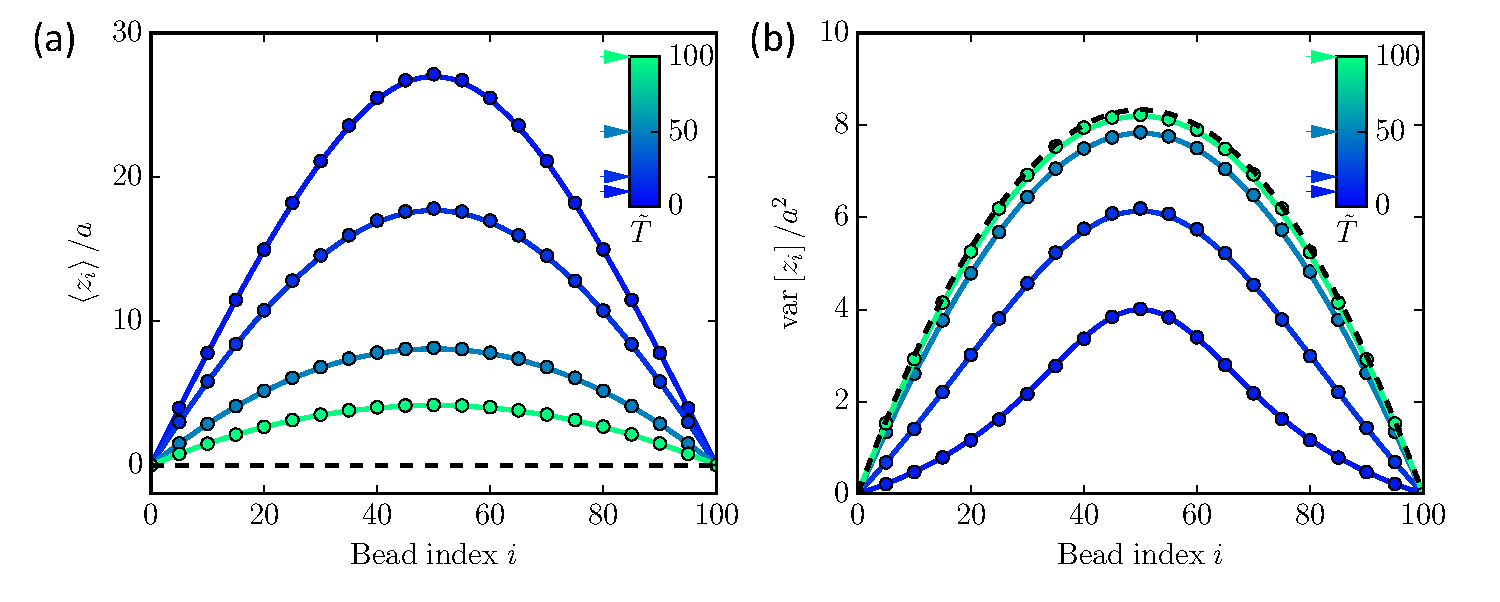
\includegraphics[width=1.0\linewidth]{meanVarZ3D}
    \caption{Mean and variance of the bead position in the direction along the force field. Solid lines are theory and dots are Monte-Carlo simulation results. The black dash line indicates the case $\tilde{T}\rightarrow\infty$, i.e. no external force field.}
    \label{fig:meanVarZ3D}
\end{figure}

Now let us discuss the directions perpendicular to the force direction. By symmetric reasons, we can immediately conclude that the statistics in $x$ and $y$ directions are identical. In addition, the mean position in both direction should be vanished because there is no bias. We can write as
\begin{equation}
    \label{eq:xyMean}
    \left<x_k\right> = \left<y_k\right> = 0.
\end{equation}

On the other hand, using Eq. \eqref{eq:second_moment}, the variance of $x$ and $y$ components of the $j^{\rm{th}}$ rod orientation can be written as
\begin{equation}
    \label{eq:xyRodVar}
    \text{var}\left[u_{j,x}\right] = \text{var}\left[u_{j,y}\right] = \left<u_{j,x}^2\right> - \left<u_{j,x}\right>^2 = (1-\left<\cos^2\theta_j\right>)/2
\end{equation}
Again, impose the Brownian bridge condition similar to Eq. \eqref{eq:varBrownianBridge3D}, the variance of $x$ and $y$ components of the bead position can be obtained. Notice the variance in $x$ and $y$ directions are different from the variance in $z$ direction. This is shown in Fig \ref{fig:xyVar3D} together with the benchmark of our theory and the Monte-Carlo simulations.

\begin{figure}[htpb]
    \centering
    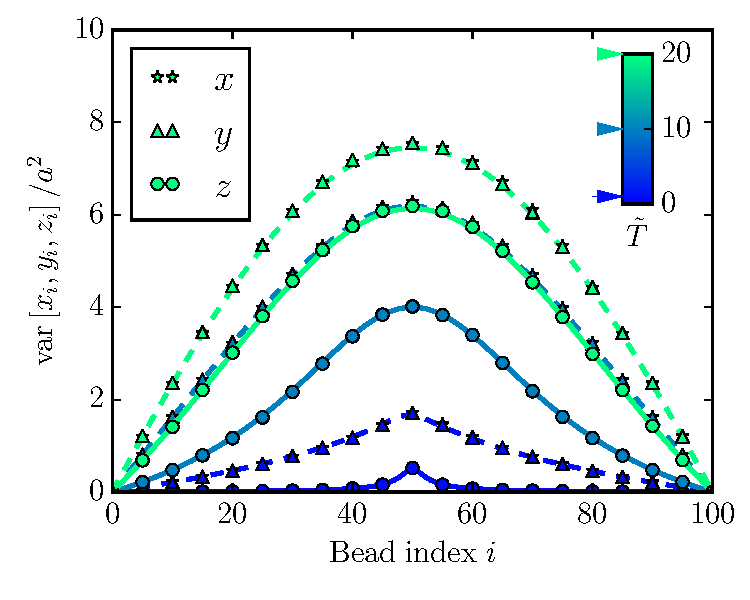
\includegraphics[width=0.8\linewidth]{xyVar3D}
    \caption{Comparison of fluctuations in $x$, $y$ and $z$ directions. Symbols denote the Monte-Carlo simulations. Circles show the fluctuations along the $z$ axis, whereas stars and triangles along $x$ and $y$ axis respectively. Colors correspond to different dimensionless temperatures. Solid and dashed lines are theoretical predictions for fluctuations along and orthogonal to the force field, respectively.}
    \label{fig:xyVar3D}
\end{figure}

In this section, we discussed the three dimensional pinned polymer loop model and its equilibrium statistics. The mean and variance of each bead position are calculated using the grand canonical ensemble combined with Brownian bridge technique. After so many discussions about the model for chromosomes, in next section, we will come back to the biological problem. Using the insight from model analysis, we will discuss the paring problem of homologous. 

%********************************** % Fourth Section  *************************************

\section{Modeling the chromosome alignment}
\label{sec:modeling_the_chromosome_alignment}
In fission yeast, the chromosomes are appearing in pairs during nuclear oscillation, which means there are two mechanically identical chromosomes. In total, there are three chromosome pairs in fission yeast. In this section, we will use the theory from the pinned polymer loop model to discuss the chromosome alignment problem in fission yeast. We will first discuss about the chromosome paring and alignment, and then fit our model to the biology.

\subsection{Chromosome paring and alignment}
\label{sub:chromosome_paring_and_alignment}

In the prophase I of fission yeast, the dramatic chromosome movements are observed before the pair of chromosomes separate into two daughter cells. However, before the separation, the pair of chromosomes are supposed to align together in space. This process is called chromosome paring, which is the necessary condition for the correct segregation later.


\begin{figure}[htpb]
    \centering
    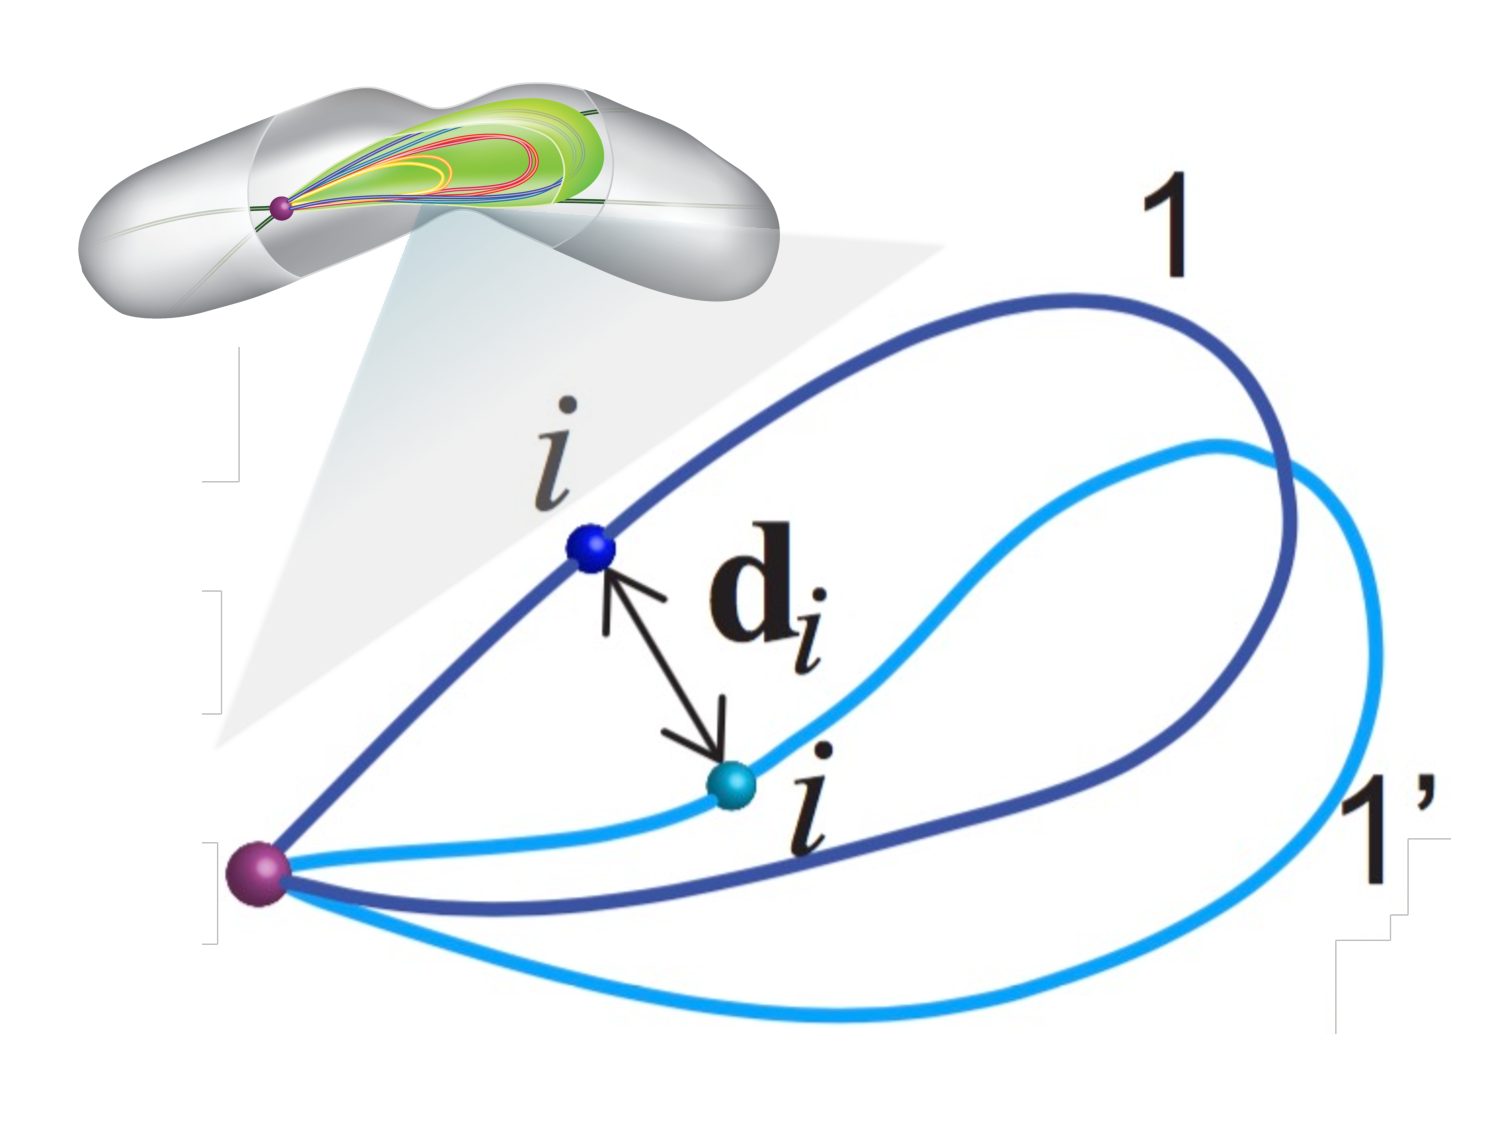
\includegraphics[width=0.6\linewidth]{pair}
    \caption{A Pair of homologous chromosomes bound to the SPB. The distance of a pair of loci is illustrated as $\mathbf{d}_i$. }
    \label{fig:pair}
\end{figure}

In the mean time of chromosome pairing, the nucleus of fission yeast is oscillating. As we discussed in Chapter $2$, the oscillation can be divided into two pieces of steady motion, which can be further transferred to the scenario of pinned polymer loop in an external force field. One can intuitively imagine that the chromosomes will be more stretched when subjecting to an stronger external force field. So the statistical distance between two corresponding loci will be shorten. Biologically, if the statistical distance is smaller than $400$nm, then it is said been paired. It is interesting to ask how does the pulling facilitate the paring of homologous. 

We will calculate the statistical distance of $\mathbf{d}_i$ (show in Fig. \ref{fig:pair}) for different external force field. 


\subsection{Theory fits to the biology}
\label{sub:theory_fits_to_the_biology}

\begin{figure}[htpb]
    \centering
    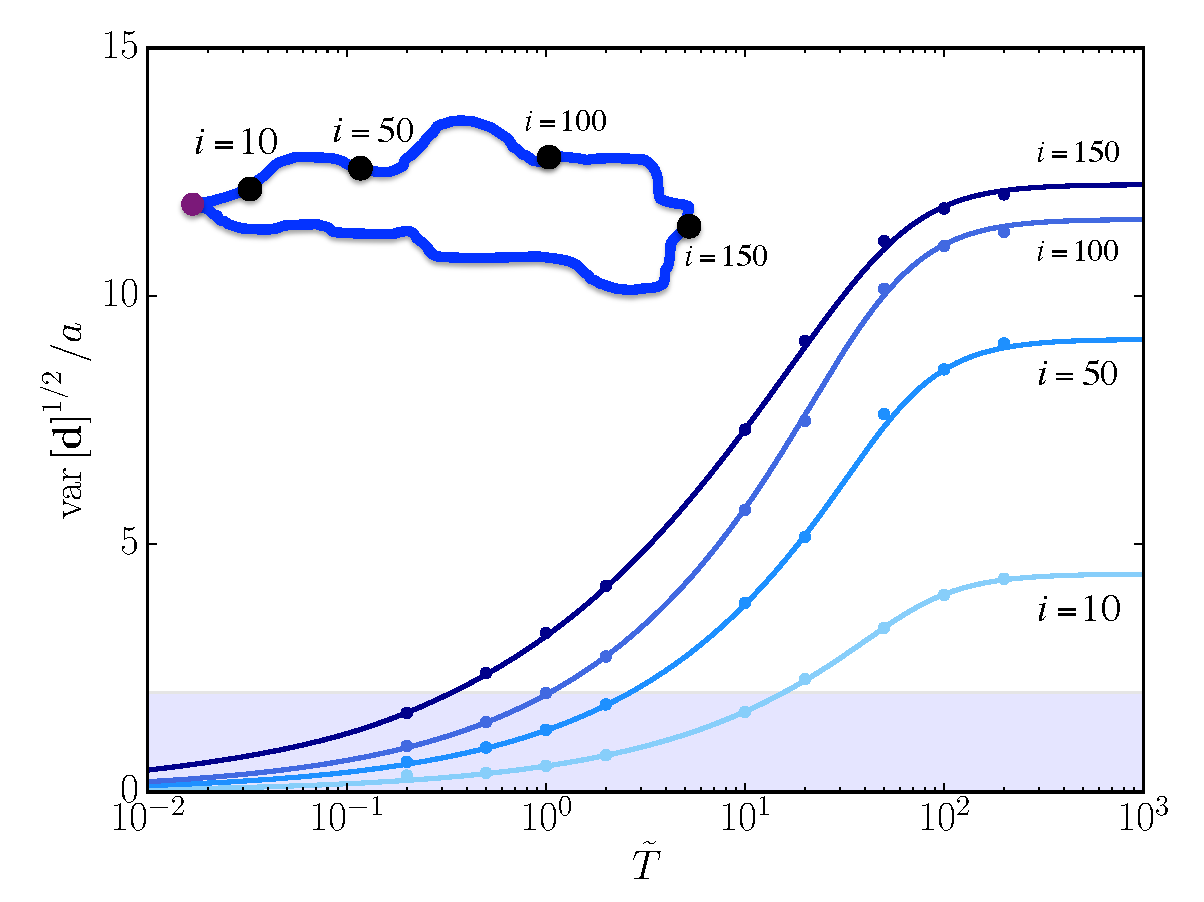
\includegraphics[width=0.8\linewidth]{paring}
    \caption{paring}
    \label{fig:paring}
\end{figure}

%********************************** % Fifth Section  *************************************

\section{Two intersecting Loops}
\label{sec:two_intersecting_loops}

\begin{figure}[htpb]
    \centering
    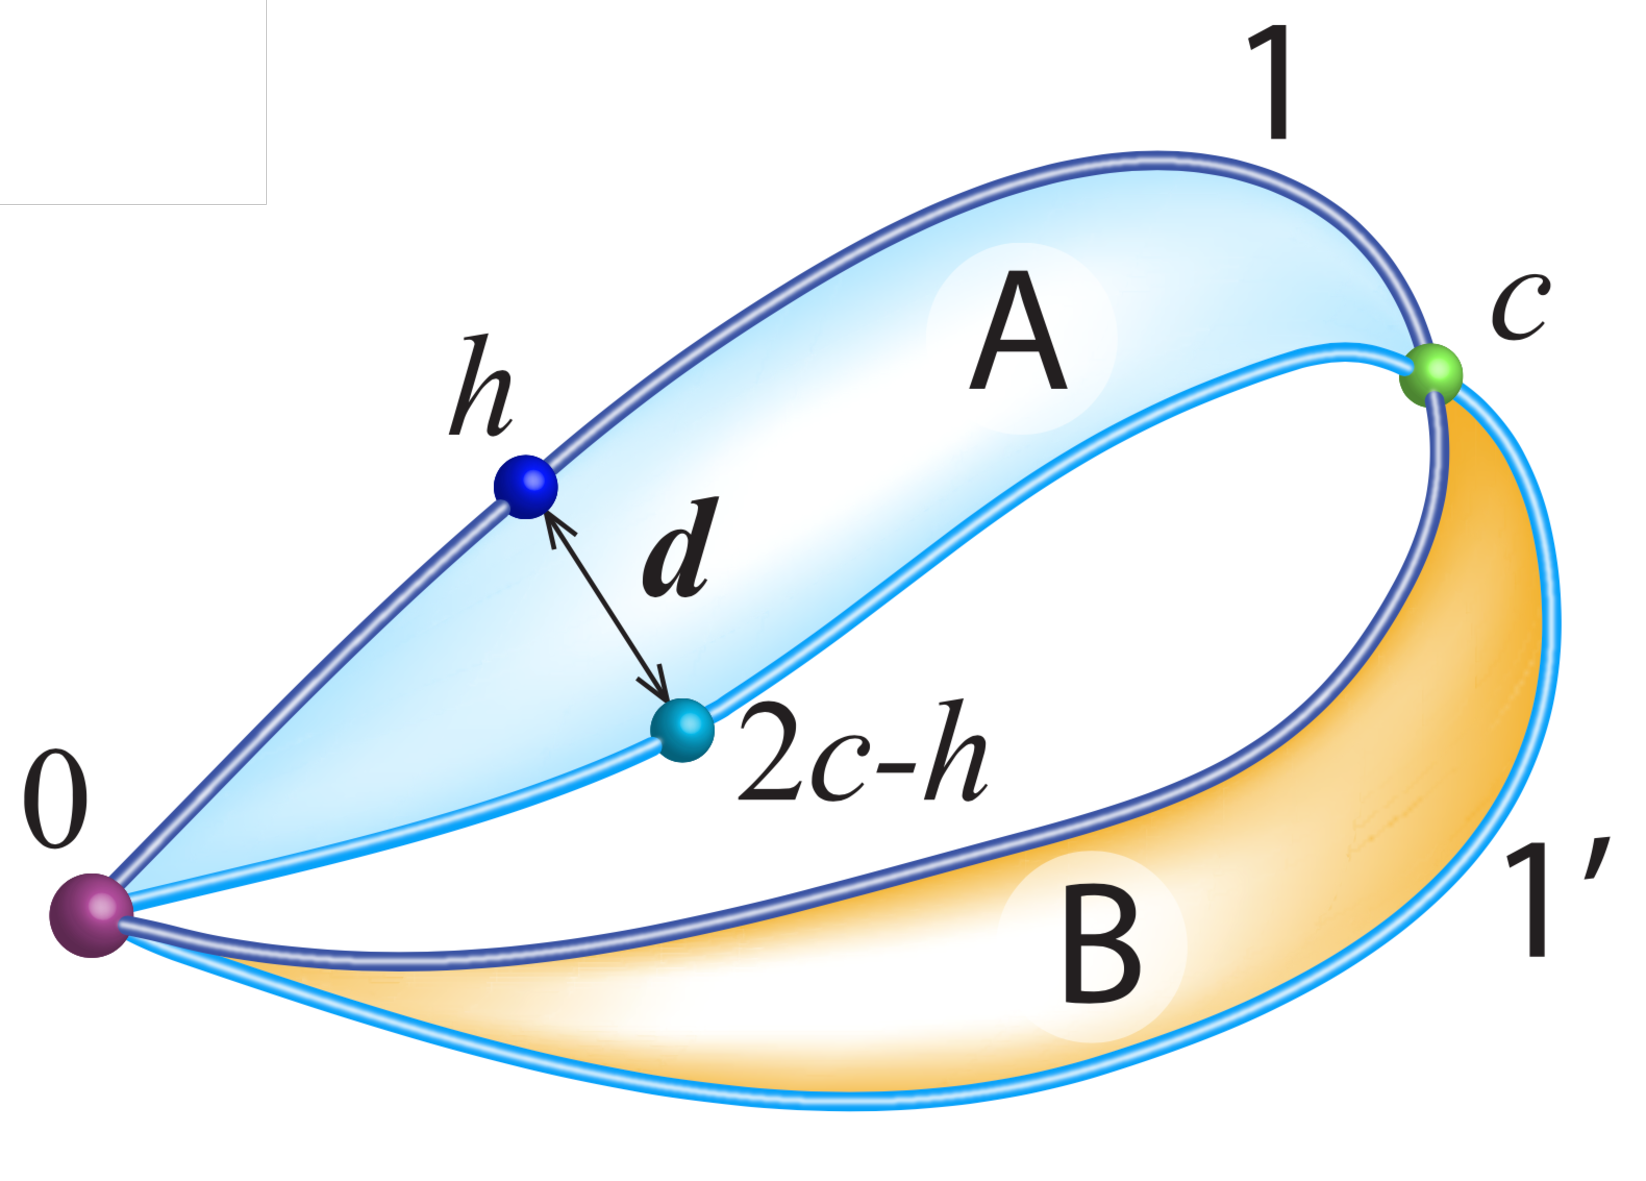
\includegraphics[width=0.6\linewidth]{centromere}
    \caption{centromere}
    \label{fig:centromere}
\end{figure}

%********************************** % Sixth Section  *************************************
\section{Summary}
\label{sec:summary_chp3}

Yen Ting Lin. 
